\chapter{Theory}\label{cha:theory}

This chapter will describe the underlying theory about the methods and algorithms used during in the automatic facial mark algorithm. 

\section{Facial landmarks} \label{sec:landmarks} 

To process a facial image, it is useful to know where different parts of the face are located, e.g. mouth and eyes. These parts can be pinpointed with points called landmarks. With these landmarks, it is possible to create a unique mask for each face and produce a grid with different regions in the face. The landmarks are extracted by using an implementation based on Vahid Kazemi et al. \cite{dlib_landmark}. It uses sate of the art algorithms for face alignment where cascade of regression functions is crucial for its success. The estimated shape of the face is updated by regressing the shape parameters based on normalized features from the image. The parameters are updated until they converge.

From this algorithm, 68 landmarks are extracted where the eyes, mouth, nose and chin are marked. From these, a mask generated where the nostrils, eyes, throat and background are cut out. 

\section{Image normalization} \label{sec:normalization} 

In order to get a reliable and uniform result in the algorithm, the facial images have to be normalized. There are two kinds of normalization applied on the image, geometric normalization and photometric normalization.  

\subsection{Geometric normalization} \label{subsec:geo_norm} 
The geometric normalization consists of rotation of the image such that the line between the pupils is aligned with the bottom of the image. The rotations angle is calculated with the help of the landmarks at the corners of the eyes. An angle is calculated by averaging an angle from the right and left eye. 

Rotation of an image is done by using a affine transformation with homogeneous coordinates \cite{li2001generalized}. Assume that a point is described as $(x, y)$ in Cartesian coordinates. Then, the point can be transformed into homogeneous coordinates such that the point is described as $(x, y, 1)$. Thanks to this coordinate system, rotation can be expressed as a simple matrix multiplication as in \cref{eq:rotation} where $(x', y', 1)$ are the rotated coordinates for a point. $\phi$ is the angle which each point is rotated counter clockwise. 

\begin{equation} \label{eq:rotation}
\begin{bmatrix}
x' \\[0.3em]
y' \\[0.3em]
1
\end{bmatrix}
=
\begin{bmatrix}
	\cos{\phi} & -\sin{\phi} & 0 \\[0.3em]
	\sin{\phi} & \cos{\phi}  & 0 \\[0.3em]
	0          & 0           & 1
\end{bmatrix}
\begin{bmatrix}
x \\[0.3em]
y \\[0.3em]
1
\end{bmatrix}
\end{equation}

The geometric normalization also includes a resize of the image such that the interpupillary distance is 500 pixels. A resizing factor is calculated by taking the fraction between 500 and the number of pixels between the pupils.  

\subsection{Photometric normalization} \label{subsec:photo_norm} 

The photometric normalization is performed by using tone mapping operator based on the work of Nikola Banic et al.\cite{badger}. It uses a Light Random Sprays Retinex (LRSR) which is an improvement of the Random Sprays Retinex (RSR)\cite{RSR}. All tone mapping operator transform pixel intensities depending on its surrounding. The RSR uses a random selection of pixels around the current pixel which decreases computations costs, sampling noise and dependency. The calculations are done on the intensity image of each RGB colour channels. An example of the output from the image normalization can be seen in \cref{fig:rotated_img}.

\section{Face detection}

An important component in the algorithm is the bounding box of the face in each image. It is found by using an OpenCV \cite{opencv} implementation of object detection by Paul Viola et al. \cite{face_detection}. This face detection algorithm was chosen since it has equivalent positive result as other methods \cite{face_detecion_comp,face_detecion_comp_2}. In addition, it is much faster the other detector. The algorithm from Paul Viola et al. take advantage of three different parts. 

The first is part is a new image representation which allows Haar features from each image to be calculated rapidly. The speed is achieved by using integral images instead of the original image. 

The second part is the extraction of the most important features through AdaBoosting. It creates a strong classifier by combining the strength of weaker classifiers. A weak classifier is the best threshold for a feature which separates the faces from the non-faces.

The third part is a cascade decision which reduces the computations costs by rejecting potential bounding boxes for the face. A simple classifier is used to determine if the bounding boxes are promising candidates before a more complex classifier is engaged. This is repeated until all classifiers has been passed or if one of the returns a negative result. All bounding boxes which has returned a negative result is rejected immediately.  

\section{Segmentation} \label{sec:segmentation} 

When searching for facial mark, hair lines and hair can cause false detection. Therefore, the image has to be segmented so that only skin area is regarded during the search of facial marks. Since interactive segmentation methods are more and more popular \cite{graphcut}, it should be beneficial to choose an interactive segmentation method. Carsten Rother et al.\cite{grabcut} compared several popular interactive segmentation methods and also presented their own method, GrabCut. They concluded that GrabCut performs as well as GraphCut \cite{graphcut} with fewer user interactions.

Thus, the segmentation method used for the algorithm is GrabCut which uses Gaussian Mixture Model (GMM) for a color image. GrabCut needs a GMM for a known foreground and one for a known background. The known foreground used e.g. is the cheeks and forehead, is extracted with the help of the landmarks. 

After creating GMM:s, an energy function is created so that its minimum correspond to a good segmentation which depends on the given foreground and background. The function is minimized iteratively until a converged segmentation is produced.

The segmentation mask is used to improve the mask created from the landmarks. Now using the improved mask, a well segmented image can be searched for facial marks. 

\section{Fast Radial Symmetry} \label{sec:FRS} 

There are many ways to extract interesting points or marks. One way is to look at the radial symmetry in the image. This method has been used by several researcher \cite{twins,FRS,automatic_detector_2015,yeast}. It seems to be a reliable method since the point is to detect small circular shapes, which is what Jan Schier et al.\cite{yeast} did when they tried to count yeast colonies. This is why the actual mark detector uses an algorithm called Fast Radial Symmetry (FRS) and it was created by Gareth Loy et al.\cite{FRS}. 

For each point, $p$, in an image, the contribution of radial symmetry at radius $r$ is calculated by producing an orientation projection image $O_n$ and a magnitude projection image $M_n$. $n$ is a specific radius. These images needs to know the so called positively-affecting pixel, $p_{+}(p)$, and negatively-affecting pixel, $p_{-}(p)$. To find theses affecting pixels the gradient, $g$, of the image is needed and it is calculated using a 3x3-Sobel kernel. Since the gradient computations are discrete, it is necessary to average the image with a 3x3 Gaussian kernel to remove sharp edges. 

\begin{equation} \label{eq:p+}
p_{+}(p) = g(p) + \text{round}\frac{g(p)}{\norm{g(p)}}n
\end{equation}

\begin{equation} \label{eq:p-}
p_{-}(p) = g(p) - \text{round}\frac{g(p)}{\norm{g(p)}}n
\end{equation}

To retrieve the nearest integer the operation $round$ is used. The $O_n$ and $M_n$ are then updated according to \cref{eq:O+,eq:O-,eq:M+,eq:M-}

\begin{equation} \label{eq:O+}
O_{n}(p_{+}) = O_{n}(p_{+}) + 1
\end{equation}
\begin{equation} \label{eq:O-}
O_{n}(p_{-}) = O_{n}(p_{-}) - 1
\end{equation}
\begin{equation} \label{eq:M+}
M_{n}(p_{+}) = M_{n}(p_{+}) + \norm{g(p)}
\end{equation}
\begin{equation} \label{eq:M-}
M_{n}(p_{-}) = M_{n}(p_{-}) - \norm{g(p)}
\end{equation}

The radial symmetry contribution at radius n depends on $F_n$ and $A_n$ which is defined as 

\begin{equation} \label{eq:F}
F_n = \frac{M_{n}(p)}{k_n} \left(\frac{\abs{\tilde{O}_n(p)}}{k_n}\right)^{\alpha}
\end{equation}
\begin{equation} \label{eq:A}
\tilde{O}_n(p) =   
\begin{cases}
O_n(p)    & \quad \text{if } O_n(p) < k_n\\
0		& \quad  \text{ else}\\
\end{cases}
\end{equation}

$A_n$ is a Gaussian kernel with different size depending on $n$, $\alpha$ is radial strictness parameter and $k_n$ is a scaling factor. $\alpha$ is set to $2$ and $k_n$ to $9.9$ since Gareth Loy et al. deemed suitable for most applications.

The final radial symmetry image $S_n$ is calculated 

\begin{equation} \label{eq:S_for_n}
S_{n} = F_n * A_n
\end{equation}

This was a calculation for radius $n$ and it desirables to use multiple radii to detect point larger than $n$. It is not necessary to use a continuous spectrum of radii according to Gareth Loy et al. The average of radial symmetry images, $S$, are then calculated as in \cref{eq:S_total}. The image S is highlighting radial symmetrical regions and suppressing regions that are asymmetrical.  

\begin{equation} \label{eq:S_total}
S =\frac{1}{N} \sum_{n=1}^{N} S_n
\end{equation}



\section{Candidate elimination} \label{sec:elimination} 

Since many facial mark candidates may be false positives, they have to be discovered and excluded. Vorder Bruegge et al. \cite{automatic_detector_2015} used three elimination methods which seemed intuitive. Size, shape and presence of hair should be good indicators if the candidate is a false detection or not. Each detected candidate is given a 30x30 area which is processed through three eliminators. 

\subsection{Blob selection} \label{subsec:blob_eli} 

Facial marks are often blob-shaped which is why the first eliminator uses a simple blob detector from OpenCV. It creates a thresholded images with connective pixels and does this with different threshold values. Each image created with a fixed threshold is put together into image which is the union of all the thresholded images. If the union does not contain a blob-shaped object, the candidate is eliminated. A blob-shaped object is defined by its circularity, inertia and convexity.  

\subsection{Hair elimination} \label{subsec:hair_eli} 

The second eliminator uses a hair removal algorithm by Tim Lee et al. \cite{dullrazor}. The algorithm smooth out hair pixels with closing operations using the three different structuring elements. The suggested structuring elements by Tim Lee et al. is larger than the one used in this implementation since their hair-structures where wider. Thus, the smaller structuring elements $T_{0}$, $T_{45}$ and $T_{90}$ were used. \\

\begin{center}
	$T_{0} =
	\left[ \begin{array}{@{}*{5}{c}@{}}
	0 & 1 & 1 & 1 & 0  \\
	\end{array} \right]  $ \quad $T_{45} =
	\left[ \begin{array}{@{}*{4}{c}@{}}
	0 & 0 & 0 & 0 \\
	0 & 1 & 0 & 0 \\
	0 & 0 & 1 & 0 \\
	0 & 0 & 0 & 0  \\
	\end{array} \right]$ \quad $T_{90} = (T_{0})^{T} $ \\
\end{center}

The closed image is generated by applying each structure element on each color channel as \eqref{eq:hair}, where $G$ is the closed image, $M$ is the image of a mark, $T_x = [T_{0}, T_{45}, T_{90} ]$ and $C$ the RGB-channels. This means that $M_c$ is a gray image of a mark where the structuring elements detect thin and small edges.    

\begin{equation} \label{eq:hair}
G_c = \abs{M_c - \max_{x}(M_c * T_x)} 
\end{equation}

$\max\limits_x(M_c * T_x)$ means that the largest pixel value from the structuring elements are pick for that color channel. In the end, the union of $G_c$ is calculated and to get a hair mask, the union is binary thresholded with $h_{hair}$. If a region contains more than a certain amount of hair pixels, it will be excluded.

\subsection{Size elimination} \label{subsec:size_eli} 

The third eliminator removes candidates depending on their size. If the candidate has an area smaller than 20 pixels or an area larger than 1000 pixels, it is eliminated. The thresholds were chosen because all annotated marks is within this interval, see \cref{fig:result_box_size}.

\FloatBarrier
\begin{figure}[!h]
	\centering
	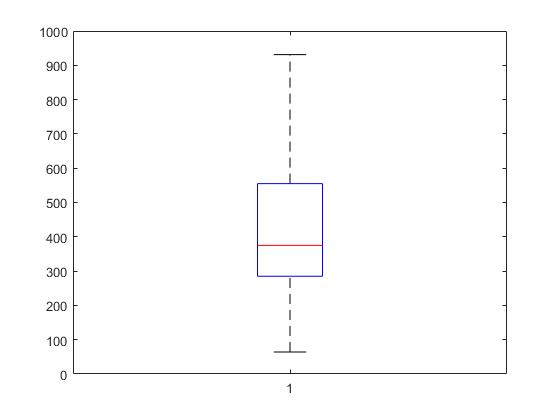
\includegraphics[width=\textwidth/2,height=\textheight/2,keepaspectratio]{result_box_size}
	\caption{The distribution of areas from the annotated facial marks.  \label{fig:result_box_size}}
\end{figure}
\FloatBarrier

\section{Machine learning} \label{sec:machine_learning} 

Machine learning is a very popular way of determining the future or sorting object into groups, e.g. whether forecast and spam filtering. The field of machine learning is growing quickly and new and more accurate methods are developed constantly. The principle is to use data to predict the outcome. The data can be somewhat incomprehensible when the dimension is getting large and abstract. This is when computers can ease the prediction by analyzing and finding patterns in the data. 

Machine learning is divided into three groups \cite{bishop2006pattern}. 

\begin{itemize}
	\item Supervised learning \\
	The system has access to labeled data from which it can find patterns and structures
	  
	\item Unsupervised learning \\
	The system does not have access to labeled data.
	
	\item Reinforcement learning \\
	The system learns from feedback given to it in form of rewards and punishments. 
\end{itemize}

A learned system can in turn be divided into two groups. 

\begin{itemize}
		\item Classification \\
		The system tries to determine the class which an object belong to, e.g. spam filtering
		
		\item Regression \\
		The system tries to predict value from an input, e.g. predicting the temperature 
\end{itemize}

This master thesis will only focus on supervised learning and classification since the desired output is permanent or non-permanent mark and there are labeled facial mark are available.  

\subsection{Supervised learning}

Supervised learning is when one try to find a function $g$ that maps $X \to \Omega$. $X$ is a vector with $N$ samples with $M$ descriptive features \cref{eq:supervised}, see \cref{sec:features}. A binary classifier usually has $\Omega = \{-1,1\}$ which it is in this case. The function $g$ takes a set of parameters $\omega = \{\omega_1 \dots \omega_K\} $ to speed up the classification of a new sample. To train the classifier, it needs training data which is a set of samples, $X$, paired with a label, $Y$. The labels has the same values as $\Omega$. 

\begin{equation} \label{eq:supervised}
X = \{x_1 \dots x_N \} \quad \text{where} \quad x_i = \{f_{i1} \dots f_{iM} \}
\end{equation}

The choice of descriptive feature a crucial for the performance of the classifier. Avrim L. Bluma et al. \cite{blum1997selection} point out importance of finding relevant and strong features. It is very easy to access to huge amount of low-quality data on the Internet. It is not the number of features that decide the performance of a classifier but rather the relevance of feature and samples. 

To illustrate how a learning method works, we jump right to a specific learning method called Support vector machine (SVM) \cite{cortes1995support}, see \cref{section:SVM} . There exist several other learning methods such as decision tree \cite{loh2011classification}, nearest neighbor \cite{keller1985fuzzy}, neural network \cite{kohonen1988introduction} and many more. This master thesis will use SVM since it is simple to use and it performed best \cite{torso_RPPVSM} compared to decision tree and nearest neighbor when classifying RPPVSM and non-RPPVSM.  


\subsection{Support vector machine} \label{section:SVM}

The principle behind SVM is to separate classes with a simple line (2D) or hyper plane (higher dimension). The line and plane can be described by its normal which has the parameters $\omega = \{\omega_1 \dots \omega_K\}$ and fulfill the equation of the plane \cref{eq:plane} where $x$ is a point on the plane and $b$ describes the distance from origin. 

\begin{equation} \label{eq:plane}
\omega^T \bullet x + b = 0 
\end{equation}

The challenge now is to find the best $\omega$ which separate the classes with the largest margin. The first attempt is a linear SVM.

\subsubsection{Linear SVM}

Vapnik et al.\cite{vapnik1963pattern} developed the linear SVM and it works like follows. Given a set of $N$ samples, $X = \{x_1 \dots x_N\}$, one want to find the normal vector $\omega = \{\omega_1 \dots \omega_K\}$ of the hyperplane which separates the two classes with the largest margin. By setting up a set of equations \cref{eq:linear_SVM} where $x_s$ is one of the samples closes to the hyperplane, so called support vector. $z_p$ is a point on the hyperplane (not a sample), $\epsilon$ is the perpendicular distance between the hyperplane and $x_s$ and $b$ determines the offset of the hyperplane from the origin along $w$. 

\begin{equation} \label{eq:linear_SVM}
\begin{cases}
\omega^T \bullet x_s + b =1\\
x_s = z_p + \epsilon \hat{\omega} \\
\end{cases}
\end{equation}

\begin{equation} \label{eq:linear_SVM_simple}
\begin{split}
& \omega^T \bullet (z_p + \epsilon \hat{\omega}) + b = 1  \iff \\
& \epsilon \omega^T \bullet \hat{\omega} + \omega^T \bullet z_p + b = 1 \iff \\
& \backslash \omega^T \bullet \hat{\omega} = \norm{\omega} \:\:  \text{and} \:\: \omega^T \bullet z_p + b = 0  \backslash \\
& \epsilon \norm{\omega} = 1
\end{split}
\end{equation} 

After some manipulation, see \cref{eq:linear_SVM_simple}, one notice that the best margin $\epsilon$ is achieved by minimizing $\norm{\omega}$ which is the same as minimizing $\norm{\omega}^2$ . When finding the maximal $\epsilon$, no samples may reside within the margin which can be expressed as \cref{eq:linear_SVM_in_margin} where $y_i$ is the class for each sample. This give the best hyperplane for the classifier where the classes are linearly separable \cref{fig:easy_class}.

\begin{equation} \label{eq:linear_SVM_in_margin}
y_i(\omega^T \bullet x_i + b) \geq 1
\end{equation} 

\FloatBarrier
\begin{figure}[!h]
	\centering
	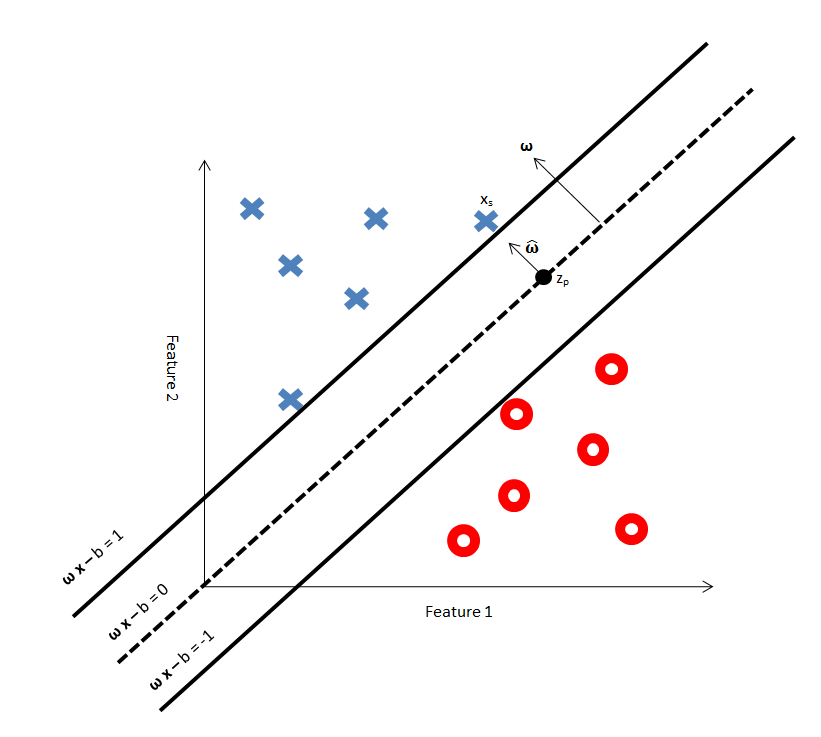
\includegraphics[width=\textwidth*3/4,height=\textheight*3/4,keepaspectratio]{easy_svm.PNG}
	\caption{Linearly separable classes.
		\label{fig:easy_class}}
\end{figure} 
\FloatBarrier


\subsubsection{Soft margin SVM}

All classification problems are not always linearly separable. In this case, \cref{eq:linear_SVM_in_margin} does not hold true for all samples. This is solved by introducing a penalty $\zeta$ \cite{cortes1995support} for each sample on the wrong side of the hyperplane. This type of SVM is called a soft margin SVM. In this type, one try to solve \cref{eq:soft_SVM} where $C$ is a parameters set before optimization. 

\begin{equation} \label{eq:soft_SVM}
\underset{\omega,b,\zeta}{\mathrm{\argmin}} 
\begin{pmatrix}
\norm{\omega}^2 + C\sum_{i}\zeta_i
\end{pmatrix}
\end{equation} 

under the condition \cref{eq:soft_SVM_2}

\begin{equation} \label{eq:soft_SVM_2}
y_i(\omega^T \bullet x_i + b) \geq 1 - \zeta \quad \zeta \geq 0
\end{equation} 

Large values on $C$ results in a greater penalization for wrongly classified samples. This parameter makes a tradeoff between having a large margin and allowing samples to be on the wrong side of the hyperplane.    

\FloatBarrier
\begin{figure}[!h]
	\centering
	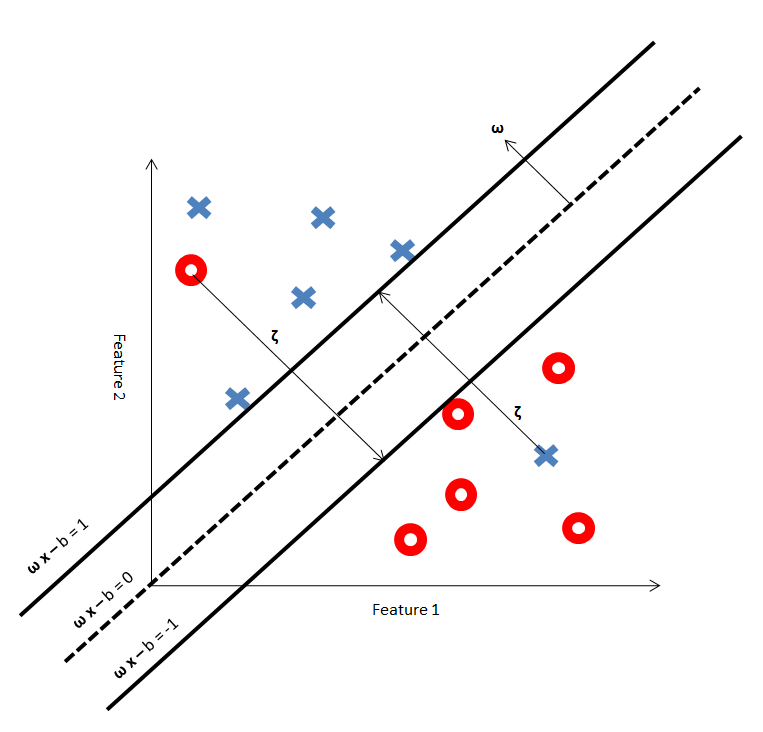
\includegraphics[width=\textwidth*3/4,height=\textheight*3/4,keepaspectratio]{soft_svm.PNG}
	\caption{Classes separated by a soft margin SVM.
		\label{fig:soft_class}}
\end{figure} 
\FloatBarrier

\subsubsection{Non-linear SVM}

Things are not always as simple as the case in \cref{fig:easy_class,fig:soft_class}. The classes are often not linearly separable at all. Fig. \ref{fig:hard_class} illustrate the so called XOR problem \cite{yu2012svm}. This classification problem requires a non-linear SVM. Boster et al. \cite{boser1992training} presented a way to solve the XOR problem by mapping the samples onto a higher dimension. This is done by using kernels, $k(x_i,x_j)$, of different types \cite{yu2012svm}. The following are popularly used kernels: 

\begin{itemize}
	\item Polynomial: $k(x_i,x_j) =(x_i \bullet  x_j + 1)^d $
	\item Radial Basis Function (RBF): $k(x_i,x_j) = exp(-\gamma \norm{x_i - x_j}^2 $
	\item Sigmoid: $k(x_i,x_j) =\kappa x_i \bullet  x_j + c$
\end{itemize}

where $\gamma$, $d$, $\kappa$ and $c$ are parameters set by the user. This master thesis will only use the RBF kernel since it is easy to tune and the polynomial kernel has more hyperparameters which influence the complexity of the model \cite{svm_guide}. The $\gamma$ parameter defines how far the influence of a sample reaches, a small value meaning 'far' and vice versa. Read more about kernels in \cite{vert2004primer} 

\FloatBarrier
\begin{figure}[!h]
	\centering
	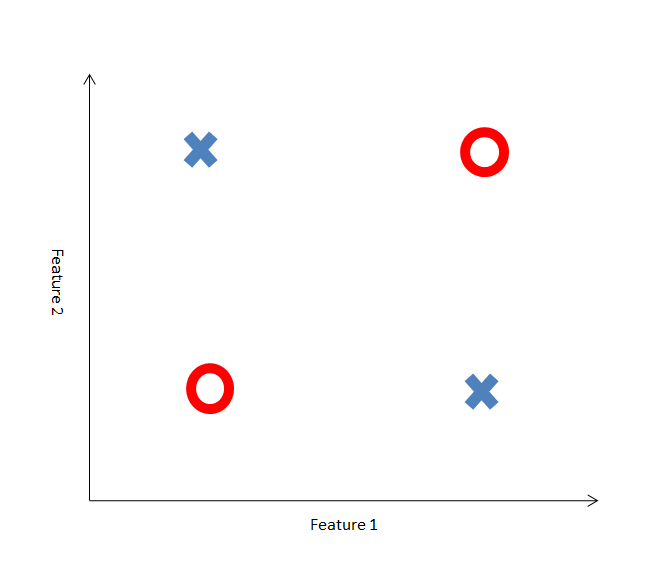
\includegraphics[width=\textwidth*2/4,height=\textheight*2/4,keepaspectratio]{hard_svm.PNG}
	\caption{XOR problem with two classes. 
		\label{fig:hard_class}}
\end{figure} 
\FloatBarrier

\subsection{Overfitting}

A large number of parameters makes it possible to produce overly complicated boundaries if the training data is used for validation. This together with usage of training data as validation data can produce a problem in machine learning known as overfitting. In \cref{fig:overfitting} one can see that the red curve is a overfitted boundary while the green curve separates the two classes more generally. Overfitting occurs when the classifier tries to include outliers or wrongly labeled samples within the classifier boundary. To avoid this, one should use a subset of all the samples as testing data which will indicate if the classifier is overtrained. 

\FloatBarrier
\begin{figure}[!h]
	\centering
	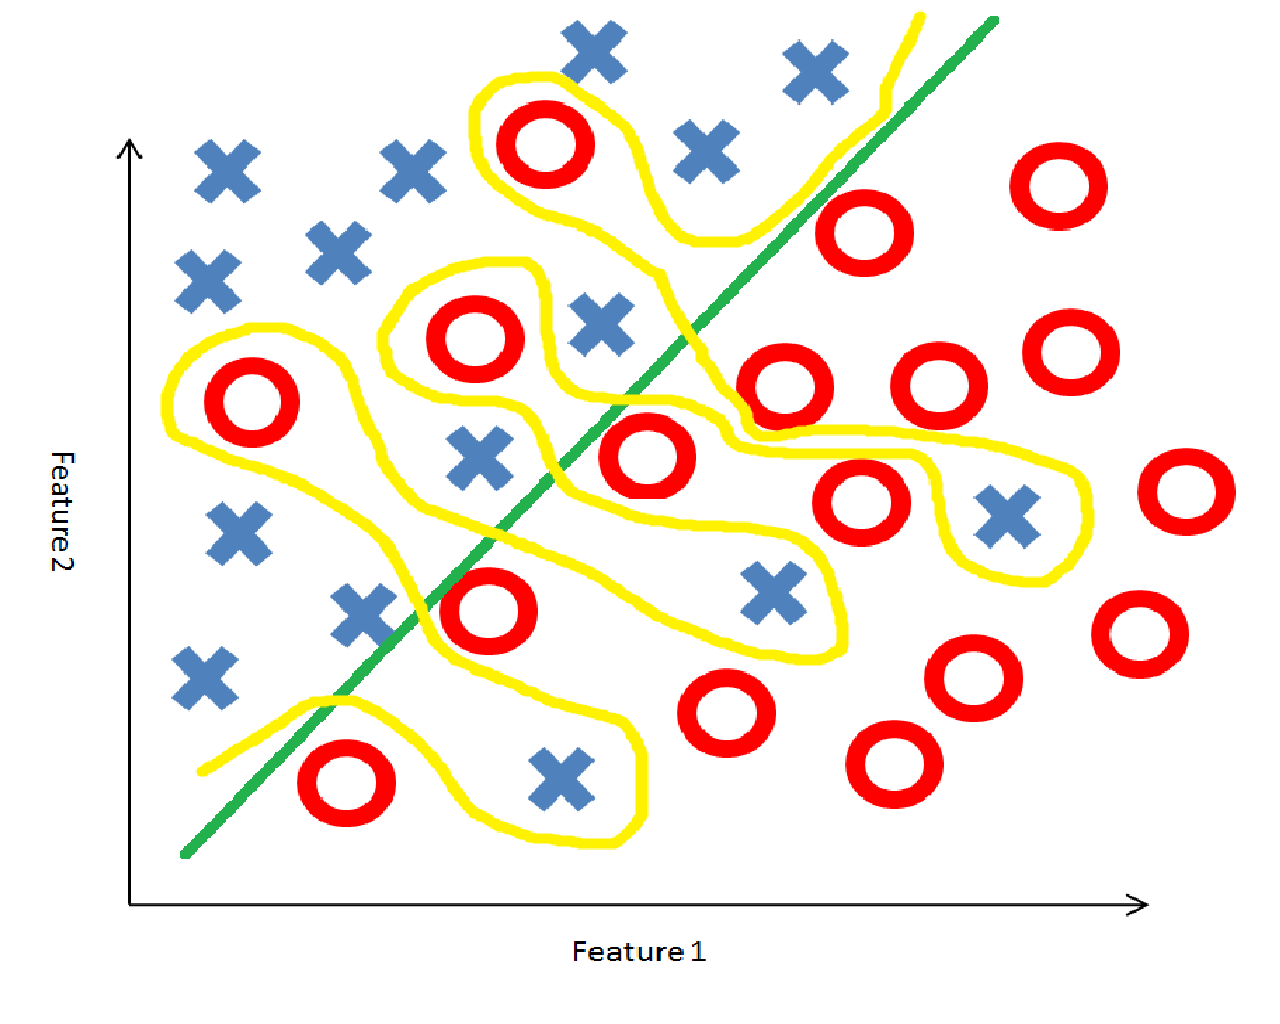
\includegraphics[width=\textwidth*2/4,height=\textheight*2/4,keepaspectratio]{Overfitting.PNG}
	\caption{Example of a overfitted boundary (yellow) and a more general boundary (green). 
		\label{fig:overfitting}}
\end{figure} 
\FloatBarrier

\section{Features descriptors} \label{sec:features}

A feature descriptor extract information about patterns in an image, in this case a facial mark. This information can consist of colors in the image, edges for distinguishing light and dark areas, the texture of a surface and the direction of movement. The feature descriptors HOG, \cref{subsection:HOG}, and LBP, \cref{subsection:LBP} are common descriptors when working with detection of objects \cite{pedestrian_detection,vehicle_hog,facedetection_LBP} which is why these feature are used. Since facial marks mostly differ in color rather than shape \cite{torso_RPPVSM}, it would be wise to use features which are based on the color of the skin marks. RGB and HSV, \cref{subsection:RGB_HSV}, are primitive color-mapping but has been used a feature descriptors before \cite{torso_RPPVSM}. It would be even better to use more colors than just RGB and HSV color space. Color names, \cref{subsection:Color}, are linguistic color labels given to a single pixel \cite{11_colours}. By using even more colors to describe the facial marks it should result in better classification results. 

\subsection{Histogram of Oriented Gradients} \label{subsection:HOG}

Histogram of Oriented Gradients (HOG) was introduced by Dalal and Triggs \cite{hog_dalal} and it showed that it outperformed the current feature descriptors at that time. 

The main idea of HOG is that a local object can be characterized by the edge directions of the object. The implementation of the descriptor is dividing each image into cells containing 4x4 pixels each. The orientation and magnitude of the gradient vectors is then calculated in each cell. The gradient was calculated using a simple 1-D 
$\left[ \begin{array}{@{}*{3}{c}@{}}
	-1 & 0 & 1  \\
\end{array} \right]$ Sobel kernel, \cref{eq:gradient}, without any Gaussian filtering beforehand since it only reduced the performance of the descriptor. The gradient vectors are then sorted into nine different bins ranging from $0-180^{\circ}$. This results in a histogram from each cell which is what is used as a descriptor. For better invariance to illumination, the descriptor vector should be normalized. This is done by grouping four cells into blocks. The cells in each block are concatenated, creating a vector, $v$, with the length 36. This vector is then normalized as in \cref{eq:L2_norm}. Here, $\epsilon$ is a small constant. 

\begin{equation} \label{eq:gradient}
\nabla I = I * \left[ \begin{array}{@{}*{3}{c}@{}}
-1 & 0 & 1  \\
\end{array} \right]
\end{equation}

\begin{equation} \label{eq:L2_norm}
v_{norm} = \frac{v}{\sqrt{\norm{v}^2 + \epsilon^2}}
\end{equation}

Dalal and Triggs also showed that the performance of the descriptors increased even further if the block steps was made such that the blocks overlaps 50\%. This overlapping can be observed in \cref{fig:hog_features}. The window size which Navneet Dalal et al. used was 128x64 but since facial marks are more or less cylindrical, a window size of 48x48 was used in the master thesis. 

\FloatBarrier
\begin{figure}[!h]
	\centering
	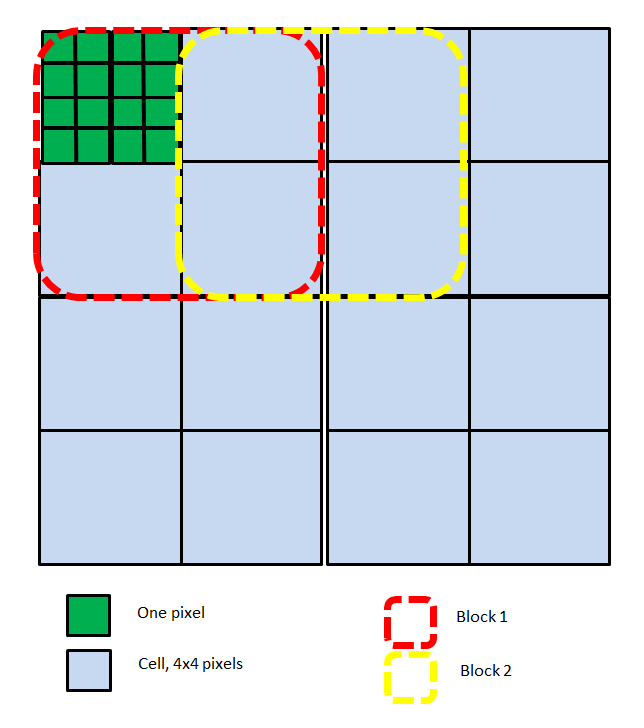
\includegraphics[width=\textwidth*2/4,height=\textheight*2/4,keepaspectratio]{hog_features.PNG}
	\caption{Schematic picture of the implementation of the HOG descriptor.
		\label{fig:hog_features}}
\end{figure} 
\FloatBarrier

\subsection{Local Binary Patterns} \label{subsection:LBP}

Local Binary Patterns (LBP) was developed by Timo Ojala et al. \cite{ojala_hog} by improving the work of Li Wang et al. \cite{pre_hog}. Li Wang et al. introduced a texture analysis method so-called texture unit. From a 3x3 pixel area, the pixels surrounding the central pixel was given either the value 0, 1 or 2. Each 3x3 pixel area would thus be given 1 out of 6561 possible texture unit. The distribution of texture units over an image was called a texture spectrum.  

Timo Ojala et al. reduced the number of possible texture unit by making a binary version of the texture unit. Each surrounding pixel, $p_s$ can would instead receive 0 or 1 depending on the value of the central pixel, $p_c$. The value is decided by \cref{eq:f_LBP}. By using a binary version of the texture unit, the number of possible texture unit is instead 256. 

\begin{equation} \label{eq:f_LBP}
f(p_s) = 
 \begin{cases}
 1    & \quad \text{if } p_s \geq p_c\\
 0		& \quad  \text{ else}\\
 \end{cases}
\end{equation}

When each surrounding pixel has been given a value, \cref{fig:lbp_features} (b), the 3x3 pixel area has a binary code, e.g. 00100010, which corresponds to 34 as decimal, \cref{eq:h_LPB}.   

\begin{equation} \label{eq:h_LPB}
LBP(p_c) = \sum_{k=0}^{7} f(p)2^k
\end{equation}

\FloatBarrier
\begin{figure}[!h]
	\centering
	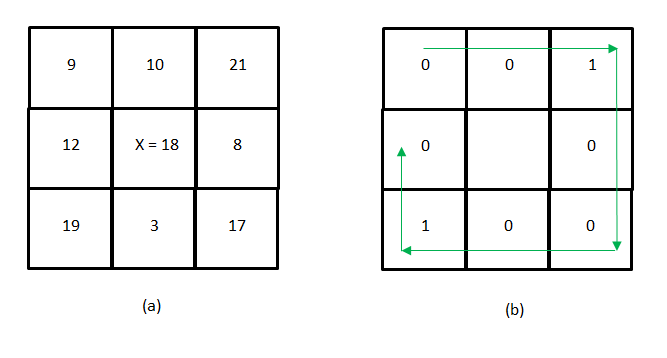
\includegraphics[width=\textwidth*3/4,height=\textheight*3/4,keepaspectratio]{lbp_features.PNG}
	\caption{Schematic picture of the implementation of the LBP descriptor. (a) Original 3x3 pixel area with x as central pixel (b) 3x3 pixel area with binary values for the surrounding pixels.
		\label{fig:lbp_features}}
\end{figure} 
\FloatBarrier

The LBP for each pixel is binned in the corresponding decimal value. This results in a 256 long vector. This vector is used a descriptive feature for the classifier. 

\subsection{RGB and HSV} \label{subsection:RGB_HSV}

RBG is the intuitive feature of choice if one want information about the color of the object. It is possible to extract much information from the color channels but this master thesis will only use the mean, $\bar{p}$ \cref{eq:mean_RGB}, and the standard deviation, $p_{\sigma}$ \cref{eq:std_RGB}, from each color channel. These values are put into a vector and are used to train the classifier.  

\begin{equation} \label{eq:mean_RGB}
\bar{p} = \frac{1}{N}\sum_{i = 1}^{N} p_i
\end{equation}

\begin{equation} \label{eq:std_RGB}
p_{\sigma} = \sqrt{\frac{1}{N}\sum_{i = 1}^{N}(p_i - \bar{p})^2}
\end{equation}

Similarly, the mean and standard deviation are extracted from the Hue, Saturation, and Value (HSV) color space \cite{hsv_color}. HSV color space is a common cylindrical-coordinate representation of the RGB color space. It was developed to be more intuitive color representation than the RGB color space.  

\subsection{Color names} \label{subsection:Color}

We use color names to describe our surrounding every day without thinking about it. It becomes however a challenge for computers to detect certain object with a specific color attribute, e.g. a red car. In computer vision, color names are used in search engines to retrieve demanded object with a certain color. To use color names in computer vision, the RGB color space has to be mapped to different colors. This has mainly been done by letting test subject label color chips \cite{griffin2006optimality}. The colors are to be chosen from a set of colors, usually black, blue, brown, gray, green, orange, pink, purple, red, white and yellow. These colors are the basic colors of the English language. The color mapping is derived from the labeled color chips. 

The problem with the color chip method is that the color chips are under ideal lighting on a color neutral background. This is not the case with real-world images which is why Joost van de Weijer et al. \cite{11_colours} have investigate the use of color names in images from real-world applications. They used a large data set of labeled real-world images and used probabilistic latent semantic analysis (PLSA) \cite{hofmann1999probabilistic} to model the data. This model tries to find the "meaning" of the words i a document. The model has also been used in computer vision where images take the role of documents and pixels the role of word \cite{barnard2003matching}. The "meaning" of the pixels are in this case the color. Joost van de Weijer et al. showed that color names learned from real-world image outperform color chips which is why this trained color mapping is used in this master thesis. 

\FloatBarrier
\begin{figure}[h]
	\centering
	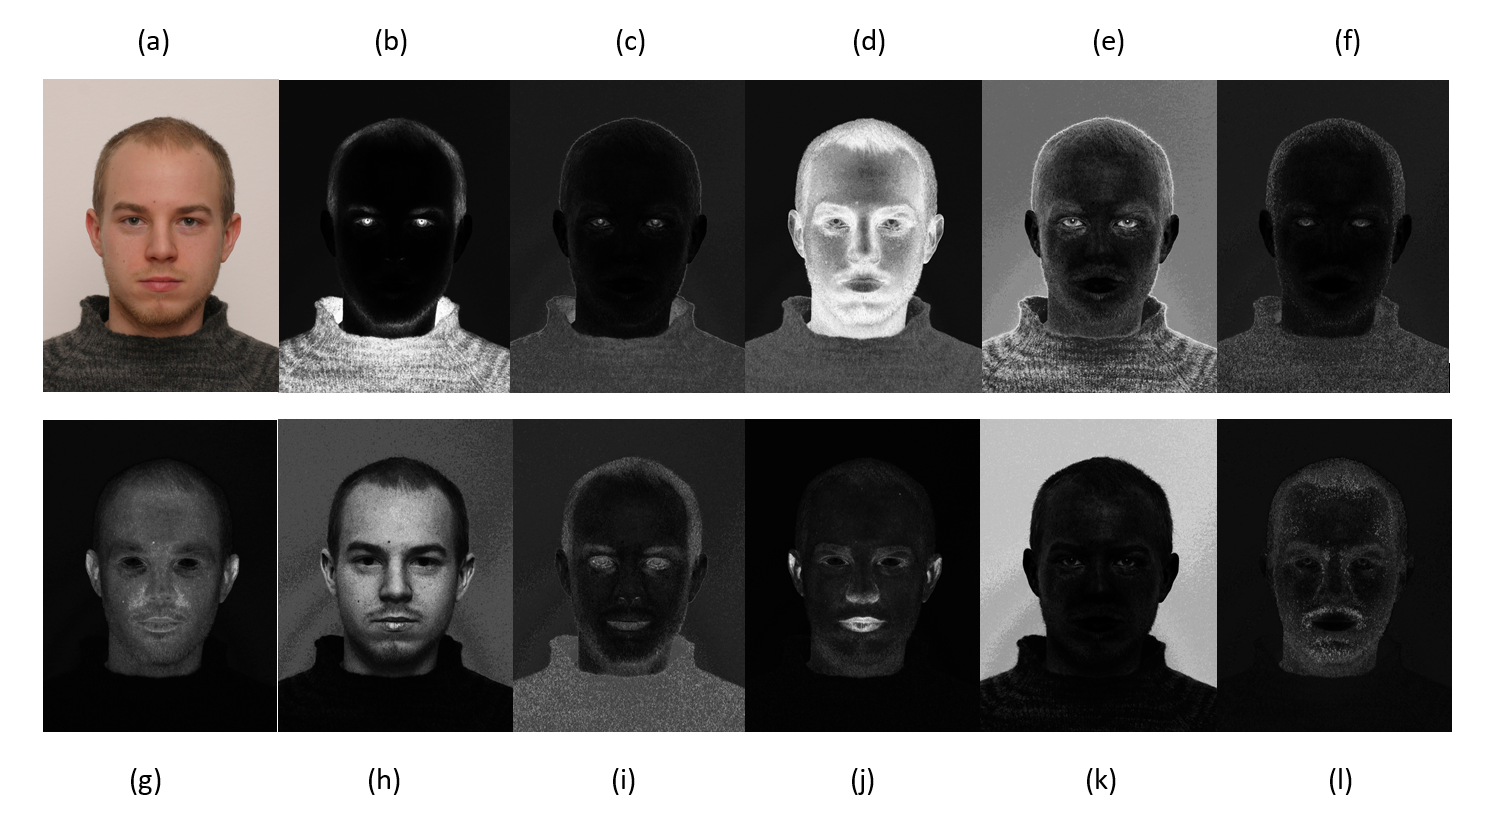
\includegraphics[width=\textwidth,height=\textheight,keepaspectratio]{faces}
	\caption{Different color channels: (a) RGB, (b) black, (c) blue, (d) brown, (e) gray, (f) green, (g) orange, (h) pink, (i) purple, (j) red, (k) white, (l) yellow  \label{fig:color_channels}}
\end{figure}
\FloatBarrier

Like the RGB and HSV color space, the mean and standard deviation is extracted from each of the 11 color names: black, blue, brown, gray, green, orange, pink, purple, red, white and yellow. 




%Resent research by Vorder Bruegge et al. \cite{automatic_detector_2015} helped the development of an automatic and semi-automatic facial mark detector. It uses a multiscale automatic facial mark detector for the automatic detector and receive a equal error rate of 15.48\%. This result was improved by introducing human knowledge in the semi-automatic detector.
%
%When distinguishing identical twins it is useful to look at facial marks which has been examined in an other article by Srinivas et al. \cite{twins}. The study concluded that the facial marks can be used as features for distinguishing between identical twins even if there seems to exist a correlations between the twins set of marks.
%
%Nurhudatiana et al. \cite{statistic_RPPVSM} describes in their article the distribution of Relatively Permanent Pigmented or Vascular Skin Marks (RPPVSM) in Caucasians, Asians, and Latinos. They conclude that if the number of RPPVSM are few they are randomly distributed which can be used for personal identification in law enforcement. 
%
%Anil and Park found during their research \cite{jain_facial} that facial mark can be used to increase the recall and precision for a state-of-the-art face matcher (FaceVACS). The facial mark detector used the 3x3 Laplacian of Gaussian-operator as blob detector. Adding these features to the algorithm improved the face matcher from  92.96\% to 93.90\% on the Facial Recognition Technology (FERET) database and from 91.88\% to 93.14\% on a Mugshot face database. 

